\chapter{Cluster membership changes}
\label{membership}

Up until now we have assumed that the cluster \emph{configuration}
(the set of servers participating in the consensus algorithm) is fixed.
In practice, it will occasionally be necessary to change the
configuration, for example to replace servers when they fail or to
change the degree of replication. This could be done
manually, using one of two approaches:
\begin{itemize}
\item Configuration changes could be done by taking the entire cluster
off-line, updating configuration files, and then restarting the cluster.
However, this would leave the cluster unavailable during the changeover.
\item Alternatively, a new server could replace a cluster member by
acquiring its network address. However, the administrator must guarantee
that the replaced server will never come back up, or else the system
would lose its safety properties (for example, there would be an extra
vote).
\end{itemize}
Both of these approaches to membership changes have significant downsides,
and if there are any manual steps, they risk operator error.

\begin{figure}
\centering
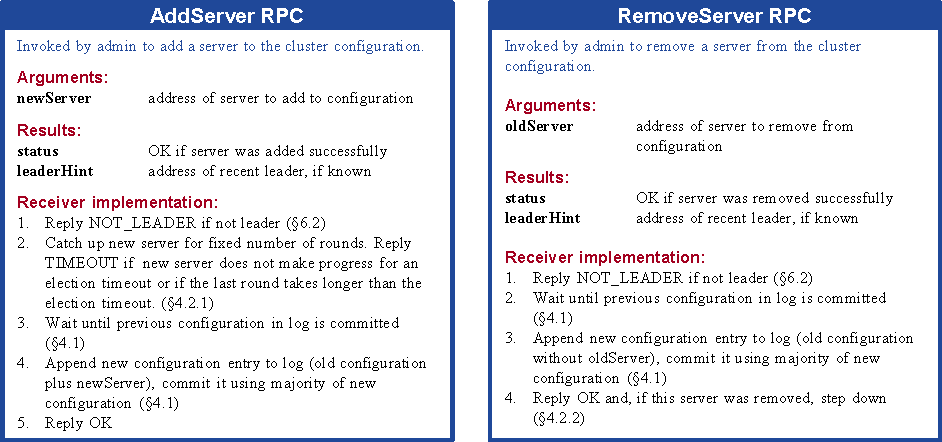
\includegraphics[scale=0.95]{membership/cheatsheet2}
\vcaption[RPCs to change cluster membership]{
RPCs used to change cluster membership. The
AddServer RPC is used to add a new server to the current configuration,
and the RemoveServer RPC is used to remove a server from the current
configuration.
Section numbers such as \S\ref{membership:safety} indicate where
particular features are discussed.
Section~\ref{membership:system} discusses ways to use
these RPCs in a complete system.
}
\label{fig:membership:cheatsheet2}
\end{figure}


In order to avoid these issues, we decided to automate configuration
changes and incorporate them into the \name{} consensus algorithm. Raft
allows the cluster to continue operating normally during changes, and
membership changes can be implemented with only a few extensions to the
basic consensus algorithm. Figure~\ref{fig:membership:cheatsheet2}
summarizes the RPCs used to change cluster membership, whose elements
are described in the remainder of this chapter.


\section{Safety}
\label{membership:safety}

Preserving safety is the first challenge for configuration changes.
For the mechanism to be safe,
there must be no point during the transition where it is possible for
two leaders to be elected for the same term. If a single configuration
change adds or removes many servers, switching the cluster directly from
the old configuration to the new configuration can be unsafe;
it isn't possible to atomically switch all of the servers at once, so 
the cluster can potentially split into two independent majorities
during the transition (see
Figure~\ref{fig:membership:reconfigurationdifficulty}).

\begin{figure}
\centering
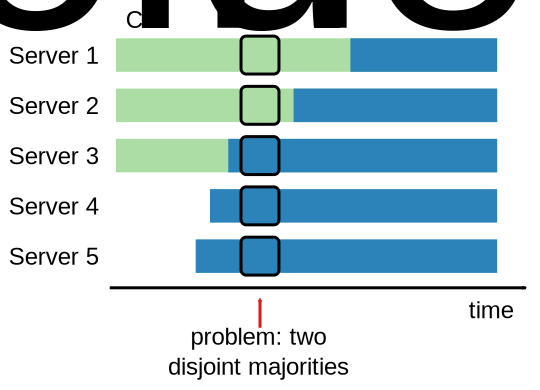
\includegraphics[scale=.50]{membership/reconfigurationdifficulty}
\vcaption[safety challenge]{
Switching directly from one configuration to another can be
unsafe because different servers will switch at different times.
In this example, the cluster grows from three servers to five.
Unfortunately, there is a point in time where two different leaders
can be elected for the same term,
one with a majority of the old
configuration (\cold{}) and another with a majority of the new
configuration (\cnew{}).
}
\label{fig:membership:reconfigurationdifficulty}
\end{figure}

\begin{figure}
\centering

\begin{subfigure}{.45\textwidth}
\centering
\includegraphics[scale=0.50]{membership/special4to5}
\caption{
Adding one server to a 4-server cluster.
}
\end{subfigure}
~
\begin{subfigure}{.45\textwidth}
\centering
\includegraphics[scale=0.50]{membership/special3to4}
\caption{
Adding one server to a 3-server cluster.
}
\end{subfigure}

\vspace{3ex}

\begin{subfigure}{.45\textwidth}
\centering
\includegraphics[scale=0.50]{membership/special5to4}
\caption{
Removing one server from a 5-server cluster.
}
\end{subfigure}
~
\begin{subfigure}{.45\textwidth}
\centering
\includegraphics[scale=0.50]{membership/special4to3}
\caption{
Removing one server from a 4-server cluster.
}
\end{subfigure}

\vcaption[adding/removing one server maintains overlap]{
The addition and removal of a single server from an even- and an
odd-sized cluster.
In each figure,
the blue rectangle shows a majority of the old cluster, and the red
rectangle shows a majority of the new cluster.
In every single-server membership change, an overlap between any majority
of the old cluster and any majority of the new cluster is preserved,
as needed for safety. For example in (b), a majority of the old cluster
must include two of the left three servers, and a majority of the new
cluster must include three of the servers in the new cluster, of which
at least two must come from the old cluster.
}
\label{fig:membership:special}
\end{figure}

Most membership change algorithms introduce additional mechanism to deal
with such problems. This is what we did for Raft initially, but we later
discovered a simpler approach, which is to disallow membership changes
that could result in disjoint majorities. Thus, Raft restricts the types
of changes that are allowed: only one server can be added or removed
from the cluster at a time. More complex changes in membership are
implemented as a series of single-server changes. Most of this chapter
describes the single-server approach, which is easier to understand than
our original approach. For completeness,
Section~\ref{membership:arbitrary} describes the original approach,
which incurs additional complexity to handle arbitrary configuration
changes. We implemented the more complex approach in LogCabin prior to
discovering the simpler single-server change approach; it still uses the
more complex approach at the time of this writing.

When adding a single server to a cluster or removing a single server
from a cluster, any majority of the old cluster overlaps with any
majority of the new cluster; see Figure~\ref{fig:membership:special}.
This overlap prevents the cluster from splitting into two independent
majorities; in terms of the safety argument of
Section~\ref{basicraft:safety:argument}, it guarantees the existence of
``the voter''. Thus, when adding or removing just a single server, it is
safe to switch directly to the new configuration. Raft exploits this
property to change cluster membership safely using little additional
mechanism.

Cluster configurations are stored and communicated using special entries
in the replicated log.
This leverages the existing mechanisms in Raft to
replicate and persist configuration information.
It also allows the cluster to continue to service
client requests while configuration changes are in progress,
by imposing ordering between
configuration changes and client requests (while allowing both to be
replicated concurrently in a pipeline and/or in batches).

When the leader receives a request to add or remove a server from its
current configuration (\cold{}), it appends the new configuration
(\cnew{}) as an entry in its log and replicates that entry using the
normal Raft mechanism. The new configuration takes effect on each server
as soon as it is added to that server's log: the \cnew{} entry is
replicated to the \cnew{} servers, and a majority of the new
configuration is used to determine the \cnew{} entry's commitment. This
means that servers do not wait for configuration entries to be
committed, and each server always uses the latest configuration found in
its log.

The configuration change is complete once the \cnew{} entry is
committed. At this point, the leader knows that a majority of the
\cnew{} servers have adopted \cnew{}. It also knows that any servers
that have not moved to \cnew{} can no longer form a majority of the
cluster, and servers without \cnew{} cannot be elected leader.
Commitment of \cnew{} allows three things to continue:
%
\begin{enumerate}
%
\item The leader can acknowledge the successful completion of the
configuration change.
%
\item If the configuration change removed a server, that server can be
shut down.
%
\item Further configuration changes can be started. Before this point,
overlapped configuration changes could degrade to unsafe situations
like the one in Figure~\ref{fig:membership:reconfigurationdifficulty}.
%
\end{enumerate}

As stated above, servers always use the latest configuration in their
logs, regardless of whether that configuration entry has been committed.
This allows leaders to easily avoid overlapping configuration changes
(the third item above), by not beginning a new change until the previous
change's entry has committed. It is only safe to start another membership
change once a majority of the old cluster has moved to operating under
the rules of \cnew{}. If servers adopted \cnew{} only when they
learned that \cnew{} was committed, Raft leaders would have a difficult
time knowing when a majority of the old cluster had adopted it. They
would need to track which servers know of the entry's commitment, and
the servers would need to persist their commit index to disk; neither of
these mechanisms is required in Raft. Instead, each server
adopts \cnew{} as soon as that entry exists in its log, and the leader
knows it's safe to allow further configuration changes as soon as the
\cnew{} entry has been committed. Unfortunately, this decision does
imply that a log entry for a configuration change can be removed (if
leadership changes); in this case, a server must be prepared to fall
back to the previous configuration in its log.

In Raft, it is the caller's configuration that is used in reaching
consensus, both for voting and for log replication:
%
\begin{itemize}
%
\item A server accepts AppendEntries requests from a leader that
is not part of the server's latest configuration. Otherwise, a new server
could never be added to the cluster (it would never accept any log entries
preceding the configuration entry that adds the server).
%
\item A server also grants its vote to a candidate that is not
part of the server's latest configuration (if the candidate has a
sufficiently up-to-date log and a current term). This vote may
occasionally be needed to keep the cluster available. For example,
consider adding a fourth server to a three-server cluster. If one server
were to fail, the new server's vote would be needed to form a majority
and elect a leader.
%
\end{itemize}
%
Thus, servers process incoming RPC requests without consulting their
current configurations.


\section{Availability}
\label{membership:availability}

Cluster membership changes introduce several issues in preserving the
cluster's availability.
%
Section~\ref{membership:availability:catchup} discusses catching up new
servers before they're added to the cluster, so that they do not stall
commitment of new log entries;
%
Section~\ref{membership:availability:removing} addresses how to phase
out an existing leader if it is removed from the cluster; and
%
Section~\ref{membership:availability:disruptive} describes how to
prevent removed servers from disrupting the leader of the new cluster.
%
Finally, Section~\ref{membership:availability:argument} closes with an
argument for why the resulting membership change algorithm is sufficient
to preserve availability during any membership change.


\subsection{Catching up new servers}
\label{membership:availability:catchup}

\begin{figure}
\centering

\begin{subfigure}{.45\textwidth}
\centering
\includegraphics[scale=1]{membership/catchupone}
\caption{
Failure of S3 while adding S4.
}
\label{fig:membership:catchupone}
\end{subfigure}
~
\begin{subfigure}{.45\textwidth}
\centering
\includegraphics[scale=1]{membership/catchupmany}
\caption{
Adding S3--S6 in quick succession.
}
\label{fig:membership:catchupmany}
\end{subfigure}

\vcaption[how adding servers can put availability at risk]{
Examples of how adding servers with empty logs can put availability at
risk. The figures show the servers' logs in two different clusters. Each
cluster starts out with three servers, S1--S3.
%
In~\subref{fig:membership:catchupone}, S4 is added, then S3 fails. The
cluster should be able to operate normally after one failure, but it
loses availability: it needs three of the four servers to commit a new
entry, but S3 has failed and S4's log is too far behind to append new
entries.
%
In~\subref{fig:membership:catchupmany}, S4--S6 are added in quick
succession. Committing the configuration entry that adds S6 (the third
new server) requires four servers' logs to store that entry, but S4--S6
have logs that are far behind.
%
Neither cluster will be available until the new servers' logs are caught
up.
}
\end{figure}

When a server is added to the cluster, it typically will not store any
log entries. If it is added to the cluster in this state, its log could
take quite a while to catch up to the leader's, and during this time,
the cluster is more vulnerable to unavailability. For
example, a three-server cluster can normally tolerate one failure with
no loss in availability. However, if a fourth server with an empty log
is added to the same cluster and one of the original three servers
fails, the cluster will be temporarily unable to commit new entries (see
Figure~\ref{fig:membership:catchupone}). Another availability issue
can occur if many new servers are added to a cluster in
quick succession, where the new servers are needed to form a majority of
the cluster (see Figure~\ref{fig:membership:catchupmany}). In both
cases, until the new servers' logs were caught up to the leader's, the
clusters would be unavailable.

In order to avoid availability gaps, Raft introduces an additional phase
before the configuration change, in which a new server joins the cluster
as a non-voting member. The leader replicates log entries to it, but it
is not yet counted towards majorities for voting or commitment purposes.
Once the new server has caught up with the rest of the cluster, the
reconfiguration can proceed as described above. (The mechanism to
support non-voting servers can also be useful in other contexts; for
example, it can be used to replicate the state to a large number of
servers, which can serve read-only requests with relaxed consistency.)

The leader needs to determine when a new server is sufficiently caught
up to continue with the configuration change. This requires some care to
preserve availability: if the server is added too soon, the cluster's
availability may be at risk, as described above. Our goal was to keep
any temporary unavailability below an election timeout, since clients
must already be able to tolerate occasional unavailability periods of
that magnitude (in case of leader failures). Moreover, if possible, we
wanted to minimize unavailability further by bringing the new server's
log even closer to the leader's.

The leader should also abort the change if the new server is unavailable
or is so slow that it will never catch up. This check is important:
Lamport's ancient Paxon government broke down because they did not
include it. They accidentally changed the membership to consist of only
drowned sailors and could make no more progress~\cite{Lamport:1998}.
Attempting to add a server that is unavailable or slow is often a
mistake. In fact, our very first configuration change request
included a typo in a network port number; the system correctly aborted
the change and returned an error.

\begin{figure}
\centering

\begin{subfigure}{.43\textwidth}
\centering
\includegraphics[scale=0.50]{membership/catchupstart}
\caption{
Start of round 2.
}
\end{subfigure}
~
\begin{subfigure}{.48\textwidth}
\centering
\includegraphics[scale=0.50]{membership/catchupend}
\caption{
End of round 2.
}
\end{subfigure}

\vcaption[rounds in server catchup algorithm]{
To catch up a new server, the replication of entries to the new server
is split into rounds. Each round completes once the new server has all
of the entries that the leader had in its log at the start of the round.
By then, however, the leader may have received new entries; these are
replicated in the next round.
}
\label{fig:membership:catchup}
\end{figure}

We suggest the following algorithm to determine when a new server is
sufficiently caught up to add to the cluster. The replication of entries
to the new server is split into rounds, as shown in
Figure~\ref{fig:membership:catchup}.
Each round replicates all the log entries present in the leader's log at
the start of the round to the new server's log. While it is replicating
entries for its current round, new entries may arrive at the leader; it
will replicate these during the next round. As progress is made, the
round durations shrink in time. The algorithm waits a fixed number of
rounds (such as 10). If the last round lasts less than an election
timeout, then the leader adds the new server to the cluster, under the
assumption that there are not enough unreplicated entries to create a
significant availability gap. Otherwise, the leader aborts the
configuration change with an error. The caller may always try again (it
will be more likely to succeed the next time, since the new server's log
will already be partially caught up).

As the first step to catching up a new server, the leader must discover
that the new server's log is empty. With a new server, the consistency
check in AppendEntries will fail repeatedly until the leader's
\emph{nextIndex} finally drops to one. This back-and-forth might be the
dominant factor in the performance of adding a new server to the cluster
(after this phase, log entries can be transmitted to the follower with
fewer RPCs by using batching). Various approaches can make
\emph{nextIndex} converge to its correct value more quickly, including
those described in Chapter~\ref{basicraft}. The simplest approach to
solving this particular problem of adding a new server, however, is to
have followers return the length of their logs in the AppendEntries
response; this allows the leader to cap the follower's \emph{nextIndex}
accordingly.

\subsection{Removing the current leader}
\label{membership:availability:removing}


If the existing leader is asked to remove itself from the cluster, it
must step down at some point. One straightforward approach is to use
the leadership transfer extension described in Chapter~\ref{basicraft}:
a leader that is asked to remove itself would transfer its leadership to
another server, which would then carry out the membership change normally.

We initially developed a different approach for Raft, in which the
existing leader carries out the membership change to remove itself, then
it steps down. This puts Raft in a somewhat awkward mode of operation
while the leader temporarily manages a configuration in which it is not
a member. We initially needed this approach for arbitrary configuration
changes (see Section~\ref{membership:arbitrary}), where the old
configuration and the new configuration might not have any servers in
common to which leadership could be transferred. The same approach is
also viable for systems that do not implement leadership transfer.

\begin{figure}
\centering
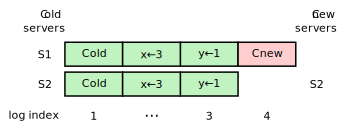
\includegraphics[scale=1]{membership/removedlog3}
\vcaption[example of progress depending on removed server]{
Until the \cnew{} entry has been committed, a removed server
may need to lead the cluster to make progress.
The figure shows the removal of S1 from a two-server cluster. S1
is currently leader. S1 should not step down quite yet; it is
still needed as leader. S2 cannot become leader until it receives the
\cnew{} entry from S1 (since S2 still needs S1's vote to form a majority
of \cold{}, and S1 won't grant its vote to S2 because S2's log is less
up-to-date).
}
\label{fig:membership:removedlog3}
\end{figure}

In this approach, a leader that is removed from the configuration steps
down once the \cnew{} entry is committed. If the leader stepped down
before this point, it might still time out and become leader again,
delaying progress. In an extreme case of removing the leader from a
two-server cluster, the server might even have to become leader again
for the cluster to make progress; see
Figure~\ref{fig:membership:removedlog3}. Thus, the leader waits until
\cnew{} is committed to step down. This is the first point when the new
configuration can definitely operate without participation from the
removed leader: it will always be possible for the members of \cnew{} to
elect a new leader from among themselves.
%
After the removed leader steps down, a server in \cnew{} will time out
and win an election. This small availability gap should be tolerable,
since similar availability gaps arise when leaders fail.

This approach leads to two implications about decision-making that are
not particularly harmful but may be surprising.
%
%
First, there will be a period of time (while it is committing
\cnew{}) when a leader can manage a cluster that does not include
itself; it replicates log entries but does not count itself in
majorities.
%
Second,
a server that is not part of its own latest configuration should
still start new elections, as it might still be needed  until the
\cnew{} entry is committed (as in
Figure~\ref{fig:membership:removedlog3}). It does not count its own vote
in elections unless it is part of its latest configuration.
%

\subsection{Disruptive servers}
\label{membership:availability:disruptive}

Without additional mechanism, servers not in \cnew{} can disrupt the
cluster.
Once the cluster leader has created the \cnew{} entry,
a server that is not in \cnew{} will no longer receive heartbeats, so it
will time out and start new elections.
Furthermore, it will not receive the \cnew{} entry or learn of that
entry's commitment,
so it will not know that it has been removed from the cluster.
The server will send RequestVote
RPCs with new term numbers, and this will cause the current leader to
revert to follower state. A new leader from \cnew{} will eventually be
elected, but the disruptive server will time out again and the process
will repeat, resulting in poor availability. If multiple servers have
been removed from the cluster, the situation could degrade further.


Our first idea for eliminating disruptions was that, if a server is
going to start an election, it would first check that it wouldn't be
wasting everyone's time---that it had a chance to win the election.
This introduced a
new phase to elections, called the Pre-Vote phase. A candidate would
first ask other servers whether its log was up-to-date enough to get
their vote. Only if the candidate believed it could get votes from a
majority of the cluster would it increment its term and start a normal
election.

\begin{figure}
\centering
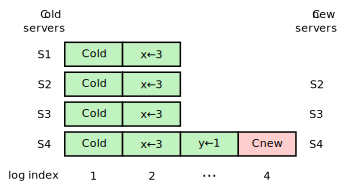
\includegraphics[scale=1]{membership/disruptive}
\vcaption[example of disruptive server]{
An example of how a server can be disruptive even before the \cnew{} log
entry has been committed, and the Pre-Vote phase doesn't help.
The figure shows the removal of S1 from a
four-server cluster. S4 is leader of the new
cluster and has created the \cnew{} entry in its log, but it hasn't yet
replicated that entry. Servers in the old cluster no longer receive
heartbeats from S4. Even before \cnew{} is committed, S1 can time out,
increment its term, and send this larger term number to the new cluster,
forcing S4 to step down. The Pre-Vote algorithm does not help, since
S1's log is as up-to-date as a majority of either cluster.
}
\label{fig:membership:disruptive}
\end{figure}

Unfortunately, the Pre-Vote phase does not solve the problem of
disruptive servers: there are situations where the disruptive server's
log is sufficiently up-to-date, but starting an election would still be
disruptive. Perhaps surprisingly, these can happen even before the
configuration change completes. For example,
Figure~\ref{fig:membership:disruptive} shows a server that is being
removed from a cluster. Once the leader creates the \cnew{} log entry,
the server being removed could be disruptive. The Pre-Vote check does
not help in this case, since the server being removed has a log that is
more up-to-date than a majority of either cluster. (Though the Pre-Vote
phase does not solve the problem of disruptive servers, it does turn out
to be a useful idea for improving the robustness of leader election in
general; see Chapter~\ref{leaderelection}.)

Because of this scenario, we now believe that no solution based on
comparing logs alone (such as the Pre-Vote check)
will be sufficient to tell if an election will be
disruptive. We cannot require a server to check the logs of
\emph{every} server in \cnew{} before starting an election,
since Raft must always be able to tolerate
faults. We also did not want to assume that a leader will reliably
replicate entries fast enough to move past the scenario shown in
Figure~\ref{fig:membership:disruptive} quickly; that might have worked
in practice, but it depends on stronger assumptions that we prefer to
avoid about the performance of finding where logs diverge and the
performance of replicating log entries.

Raft's solution uses heartbeats to determine when a valid leader exists.
In Raft, a leader is considered
active if it is able to maintain heartbeats to its followers (otherwise,
another server will start an election). Thus, servers should not be able
to disrupt a leader whose cluster is receiving heartbeats.
We modify the RequestVote RPC to achieve this: if a server receives a
RequestVote request within the minimum election timeout of hearing from a
current leader, it does not update its term or grant its vote. It can
either drop the request, reply with a vote denial, or delay the request;
the result is essentially the same. This does not affect normal
elections, where each server waits at least a minimum election timeout
before starting an election. However, it helps avoid disruptions from
servers not in \cnew{}: while a leader is able to get heartbeats to its
cluster, it will not be deposed by larger term numbers.

This change conflicts with the leadership transfer mechanism as
described in Chapter~\ref{basicraft}, in which a server legitimately
starts an election without waiting an election timeout.
In that case, RequestVote messages
should be processed by other servers even when they believe a current
cluster leader exists. Those RequestVote requests can include a special
flag to indicate this behavior (``I have permission to disrupt
the leader---it told me to!'').


\subsection{Availability argument}
\label{membership:availability:argument}

This section argues that the above solutions are sufficient to maintain
availability during membership changes. Since Raft's membership changes
are leader-based, we show that the algorithm will be able to maintain
and replace leaders during membership changes and that the leader(s) will
both service client requests and complete the configuration changes.
We assume, among other things, that a majority of the old configuration
is available (at least until \cnew{} is committed) and that a majority of
the new configuration is available.

\begin{enumerate}
%
\item A leader can be elected at all steps of the configuration change:
%
\begin{itemize}
%
\item If the available server with the most up-to-date log in the new
cluster has the \cnew{} entry, it can collect votes from a majority of
\cnew{} and become leader.
%
\item Otherwise, the \cnew{} entry must not yet be committed. The
available server with the most up-to-date log among both the old and new
clusters can collect votes from a majority of \cold{}
and a majority of \cnew{},
so no matter which configuration it uses, it can become leader.
%
\end{itemize}
%
\item A leader is maintained once elected, assuming its heartbeats get
through to its configuration, unless it intentionally steps down because
it is not in \cnew{} but has committed \cnew{}. 
%
\begin{itemize}
%
\item If a leader can reliably send heartbeats to its own configuration,
then neither it nor its followers will adopt a higher term: they will not time
out to start any new elections, and they will ignore any RequestVote
messages with a higher term from other servers. Thus, the leader will
not be forced to step down.
%
\item If a server that is not in \cnew{} commits the \cnew{} entry and
steps down, Raft will then elect a new leader. It is likely that this
new leader will be part of \cnew{}, allowing the configuration change to
complete. However, there is some (small) risk that the server that
stepped down might become leader again. If it was elected again, it
would confirm the commitment of the \cnew{} entry and soon step down,
and it is again likely that a server in \cnew{} would succeed the next
time.
%
\end{itemize}
%
\item The leader(s) will service client requests throughout the
configuration change.
%
\begin{itemize}
%
\item Leaders can continue to append client requests to their logs
throughout the change.
%
\item Since new servers are caught up before being added to the cluster,
a leader can advance its commit index and reply to
clients in a timely manner.
%
\end{itemize}
%
\item The leader(s) will progress towards and complete the configuration
change by committing \cnew{}, and, if necessary, stepping down to allow
a server in \cnew{} to become leader.
%
\end{enumerate}

\noindent
Therefore, under the above assumptions, the mechanisms described in this
section are sufficient to preserve availability during any membership
change.


\section{Arbitrary configuration changes using joint consensus}
\label{membership:arbitrary}

This section presents a more complex approach to cluster membership
changes that handles arbitrary changes to the configuration at one time.
For example, two servers can be added to a cluster at once, or all of
the servers in a five-server cluster can be replaced at once. This was
the first approach to membership changes that we came up with, and it is
described only for completeness. Now that we know about the simpler
single-server approach, we recommend that one instead, since handling
arbitrary changes requires extra complexity. Arbitrary changes are
typically the way membership changes are assumed to operate in the
literature, but we don't think this flexibility is needed in real
systems, where a series of single-server changes can change the cluster
membership to any desired configuration. 


To ensure safety across arbitrary configuration changes,
the cluster first switches to a transitional
configuration we call \emph{joint consensus}; once the joint consensus
has been committed, the system then transitions to the new
configuration. The joint consensus
combines both the old and new configurations:
\begin{itemize}
\item Log entries are replicated to all servers in both configurations.
\item Any server from either configuration may serve as leader.
\item Agreement (for elections and entry commitment) requires
separate majorities from \emph{both} the old and new configurations.
For example, when changing from a cluster of 3 servers to a
different cluster of 9 servers, agreement requires both 2 of
the 3 servers in the old configuration and 5 of the 9 servers in the new
configuration.
\end{itemize}
The joint consensus allows individual
servers to transition between configurations at different times
without compromising safety. Furthermore, joint
consensus allows the cluster to continue servicing client requests
throughout the configuration change.

\begin{figure}
\centering
\includegraphics[scale=.50]{membership/reconfigurationconf}
\vcaption[joint consensus timeline]{
Timeline for a configuration change using joint consensus. Dashed lines show configuration
entries that have been created but not committed, and solid lines
show the latest committed configuration entry. The leader first creates
the \cboth{} configuration entry in its log and commits it to \cboth{}
(a majority of \cold{} and a majority of \cnew{}).
Then it creates the \cnew{} entry and commits it to a majority of
\cnew{}. There is no point in time in which \cold{} and \cnew{} can
 both make decisions independently.
}
\label{fig:membership:reconfiguration}
\end{figure}

This approach extends the single-server membership change algorithm with an
intermediate log entry for the joint configuration;
Figure~\ref{fig:membership:reconfiguration} illustrates the
process. When the leader receives a request to
change the configuration from \cold{} to \cnew{}, it stores the
configuration for joint consensus (\cboth{} in the figure) as a log
entry and replicates that entry using the normal Raft mechanism. As with
the single-server configuration change algorithm, each server starts
using a new configuration as soon as it stores the configuration in its
log. This means that
the leader will use the rules of \cboth{} to determine when the log
entry for \cboth{} is committed. If the leader crashes, a new
leader may be chosen under either \cold{} or \cboth{}, depending
on whether the winning candidate has received \cboth{}.  In any
case, \cnew{} cannot make unilateral decisions during this period.

Once \cboth{} has been committed, neither \cold{} nor \cnew{}
can make decisions without approval of the other, and
the Leader Completeness Property ensures that only servers with the
\cboth{} log entry can be elected as leader.
It is now safe for the
leader to create a log entry describing \cnew{} and replicate it
to the cluster. Again, this configuration will take effect on
each server as soon as it is seen. When the \cnew{} log entry
has been committed under the rules of \cnew{}, the old configuration
is irrelevant and servers not in the
new configuration can be shut down. As shown in
Figure~\ref{fig:membership:reconfiguration},
there is no time when \cold{} and \cnew{} can both make
unilateral decisions; this guarantees safety.


The joint consensus approach could be generalized to allow a
configuration change to begin while a prior change was still in
progress. However, there would not be much practical advantage to doing
this. Instead, a leader rejects additional configuration changes when a
configuration change is already in progress (when its latest
configuration is not committed or is not a simple majority). Changes
that are rejected in this way can simply wait and try again later.

This joint consensus approach is more complex than the single-server
changes precisely because it requires transitioning to and from an
intermediate configuration. Joint configurations also require changes to
how all voting and commitment decisions are made; instead of simply
counting servers, the leader must check if the servers form a majority
of the old cluster and also form a majority of the new cluster.
Implementing this required finding and changing about six comparisons in
our Raft implementation~\cite{logcabin}.


\section{System integration}
\label{membership:system}

Raft implementations may expose the cluster membership change mechanism
described in this chapter in different ways. For example, the AddServer
and RemoveServer RPCs in Figure~\ref{fig:membership:cheatsheet2} can be
invoked by administrators directly, or they can be invoked by a script
that uses a series of single-server steps to change the configuration in
arbitrary ways.

It may be desirable to invoke membership changes automatically in
response to events like server failures. However, this should only be
done according to a reasonable policy. For example, it can be dangerous
for the cluster to automatically remove failed servers, as it could then
be left with too few replicas to satisfy the intended durability and
fault-tolerance requirements. One reasonable approach is to have the
system administrator configure a desired cluster size, and within that
constraint, available servers could automatically replace failed
servers.

When making cluster membership changes that require multiple
single-server steps, it is preferable to add servers before removing
servers. For example, to replace a server in a three-server cluster,
adding one server and then removing the other allows the system to
handle one server failure at all times throughout the process. However,
if one server was first removed before the other was added, the system
would temporarily not be able to mask any failures (since two-server
clusters require both servers to be available).

Membership changes motivate a different approach to bootstrapping a
cluster. Without dynamic membership, each server simply has a static
file listing the configuration. With dynamic membership changes, the
static configuration file is no longer needed, since the system manages
configurations in the Raft log; it is also potentially error-prone
(e.g., with which configuration should a new server be initialized?).
Instead, we recommend that the very first time a cluster is created, one
server is initialized with a configuration entry as the first entry in
its log. This configuration lists only that one server; it alone forms a
majority of its configuration, so it can consider this configuration
committed. Other servers from then on should be initialized with empty
logs; they are added to the cluster and learn of the current
configuration through the membership change mechanism.

Membership changes also necessitate a dynamic approach for clients to
find the cluster; this is discussed in Chapter~\ref{clients}.

\section{Conclusion}

This chapter described an extension to Raft for handling cluster
membership changes automatically. This is an important part of a
complete consensus-based system, since fault-tolerance requirements
can change over time, and failed servers eventually need to be replaced.

The consensus algorithm must fundamentally be involved in preserving
safety across configuration changes, since a new configuration affects
the meaning of ``majority''. This chapter presented a simple approach
that adds or removes a single server at a time. These operations preserve
safety simply, since at least one server overlaps any majority during
the change. Multiple single-server changes may be composed to modify the
cluster more drastically. Raft allows the cluster to continue operating
normally during membership changes.

Preserving availability during configuration changes requires handling
several non-trivial issues. In particular, the issue of a server not in
the new configuration disrupting valid cluster leaders was surprisingly
subtle; we struggled with several insufficient solutions based on log
comparisons before settling on a working solution based on heartbeats.
